\documentclass[aspectratio=169]{beamer}
\usetheme{Copenhagen}
\usecolortheme{whale}
\usefonttheme[onlymath]{serif}
\addtobeamertemplate{footnote}{\hskip -2em}{}

\usepackage{setspace}
\usepackage{xcolor}
\usepackage{graphicx}
\usepackage{multimedia}
\usepackage{fontawesome5}
\usepackage[most]{tcolorbox}
\usepackage{empheq}
\usepackage{fancybox}
\usepackage{annotate-equations}
\usepackage{soul}
\usepackage{tikz}
\usetikzlibrary{positioning, calc, shapes.geometric, shapes.multipart, 
	shapes, arrows.meta, arrows, 
	decorations.markings, external, trees}
\tikzstyle{Arrow} = [
thick, 
decoration={
	markings,
	mark=at position 1 with {
		\arrow[thick]{latex}
	}
}, 
shorten >= 3pt, preaction = {decorate}
]

\definecolor{teel}{HTML}{00AEB3}
\definecolor{redorange}{HTML}{F26035}
\definecolor{darkred}{HTML}{8B0000}
\definecolor{darkblue}{HTML}{00008B}
\definecolor{darkgreen}{HTML}{06402B}
\definecolor{CarolinaBlue}{HTML}{4B9CD3}
\definecolor{deepsea}{HTML}{123456}
\definecolor{sharedblue}{HTML}{009292}
\definecolor{distalblue}{HTML}{490092}

\usecolortheme[named=CarolinaBlue]{structure}

\title[Synthesizing for Non-Positivity]{Synthesizing Statistical and Mathematical Models to Address Non-Positivity}
\author[PN Zivich]{Paul Zivich \\ Assistant Professor \\ Department of Epidemiology \\ University of North Carolina at Chapel Hill}
\date{May 14, 2026}

\setbeamercovered{transparent}
\setbeamertemplate{navigation symbols}{}  % gets rid of the dumb navigation symbols
\setbeamertemplate{page number in head/foot}{\insertframenumber}  % adds slide #
\setbeamertemplate{headline}{}

\newcommand\blfootnote[1]{%
	\begingroup
	\renewcommand\thefootnote{}\footnote[frame]{#1}%
	\addtocounter{footnote}{-1}%
	\endgroup
}

\AtBeginSection[]{
	\begin{frame}
		\vfill
		\centering
		\begin{beamercolorbox}[sep=8pt,center,shadow=true,rounded=true]{title}
			\usebeamerfont{title}\insertsectionhead\par%
		\end{beamercolorbox}
		\vfill
	\end{frame}
}

\begin{document}
	
\begin{frame}[plain]
	\maketitle
\end{frame}

\begin{frame}{Acknowledgments\footnote[frame]{Footnotes are for asides or references}}
	\textbf{Funding}: USA NIH: K01AI177102
	~\\~\\
	\textbf{Conflicts of Interest}: None
	~\\~\\
	\textbf{Acknowledgments}: Stephen Cole, Jess Edwards, Bonnie Shook-Sa, Eric Lofgren
	~\\~\\
	\textbf{Disclaimer}: All errors are my own
	~\\~\\
	\textbf{Publication}: Zivich et al. \textit{J Epidemiol Community Health} 2026;80:352-356
	~\\~\\
	\begin{center}
		\small
		\faEnvelope \quad pzivich@unc.edu \qquad \quad 
		\faGithub \quad pzivich \qquad \quad
		\faHashtag \quad pausalz@bsky.social
	\end{center}	
\end{frame}

\begin{frame}{Motivating Example}
	\textbf{Question}: What is the mean systolic blood pressure (SBP) in mm Hg among children and adolescents aged 2-17 in the United States?
	\\~\\~\\
	\textbf{Parameter}: $\mu := E[Y]$
	\begin{itemize}
		\item $Y_i$: SBP for unit $i$
		\item $E[\cdot]$: expected value function  
	\end{itemize}
	~\\~\\
	\textbf{Data}: NHANES 2017-2018
\end{frame}

\begin{frame}{Motivating Example}
	\textbf{Systematic Error}: SBP is missing for 44\% of children
	\begin{itemize}
		\item $R_i$: indicator of SBP being observed
	\end{itemize}
	~\\
	Extent of missingness means that estimate is sensitive to choices about missing data\footnote[frame]{While a relatively simple descriptive question, we can consider causal inference to be a missing data problem and thus link the methods used here for confounding}
	~\\~\\~\\
	A complete-case analysis assumes marginal exchangeability
	$$ E[Y] = E[Y \mid R=1] $$
\end{frame}

\begin{frame}{A More Plausible Assumption}
	SBP is missing completely at random conditional on $X$
	\begin{itemize}
		\item $X_i$: age in years
	\end{itemize}
	\begin{equation*}
		E[Y \mid X=x] = E[Y \mid X=x, R=1] \text{ for all values of } x
	\end{equation*}
	~\\
	Under this assumption, $\mu$ is identified as\footnote[frame]{Estimate with direct maximum likelihood estimator, g-computation}
	\begin{equation*}
		E[Y] = E\left[ E(Y \mid X=x, R=1) \right]
	\end{equation*}
	or a weighted average of the complete-case means within strata of $X$
\end{frame}

\begin{frame}{Implication of Exchangeability}
	\textbf{Positivity}: all unique patterns of $X$ have a nonzero probability of having $Y$ being measured
	$$ \Pr(R=1 \mid X=x) > 0 \text{ for all } x \in \mathcal{X} $$
	~\\
	Every unique age in the population has a non-zero probability of having $Y$ observed
	\begin{itemize}
		\item Statement about population
		\item Deterministic or structural positivity
	\end{itemize}
\end{frame}

\begin{frame}{Why Positivity Matters}
	\textbf{Formal}: following definition of conditional expectation
	$$ E[Y \mid X=x, R=1] = \frac{E[Y R \; I(X=x)]}{\Pr(R=1 \mid X=x) \Pr(X=x)}$$
	~\\
	\textbf{Intuitive}: need some with $X=x$ to have $Y$ observed at least sometimes so can `stand-in' for those without $Y$ measured
	\\~\\~\\
	So, \textit{positivity} comes along with \textit{exchangeability}
\end{frame}

\begin{frame}{Positivity for NHANES}
	\begin{center}
		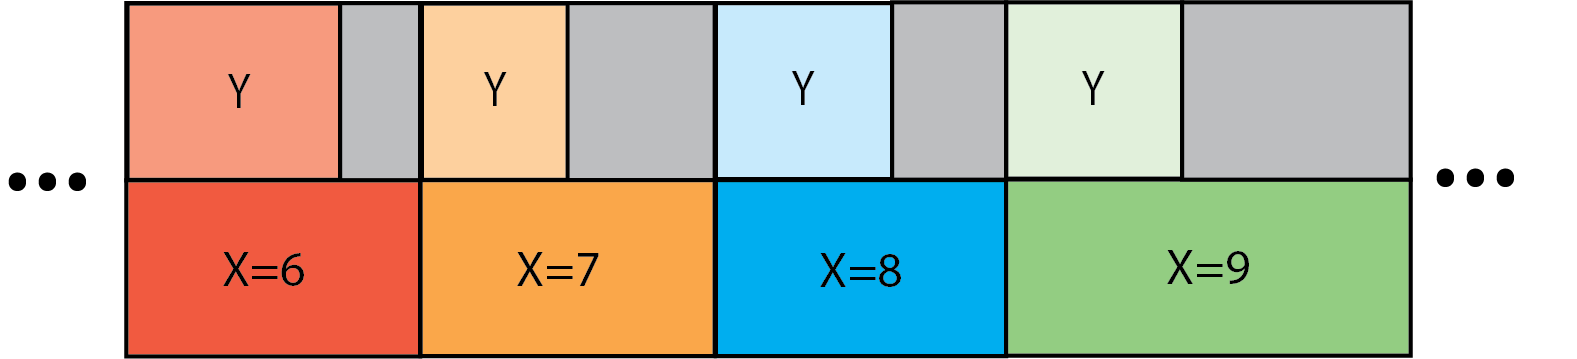
\includegraphics[width=0.85\linewidth]{images/missing-diagram1.png}
	\end{center}
\end{frame}

\begin{frame}{NHANES Data}
	\begin{center}
		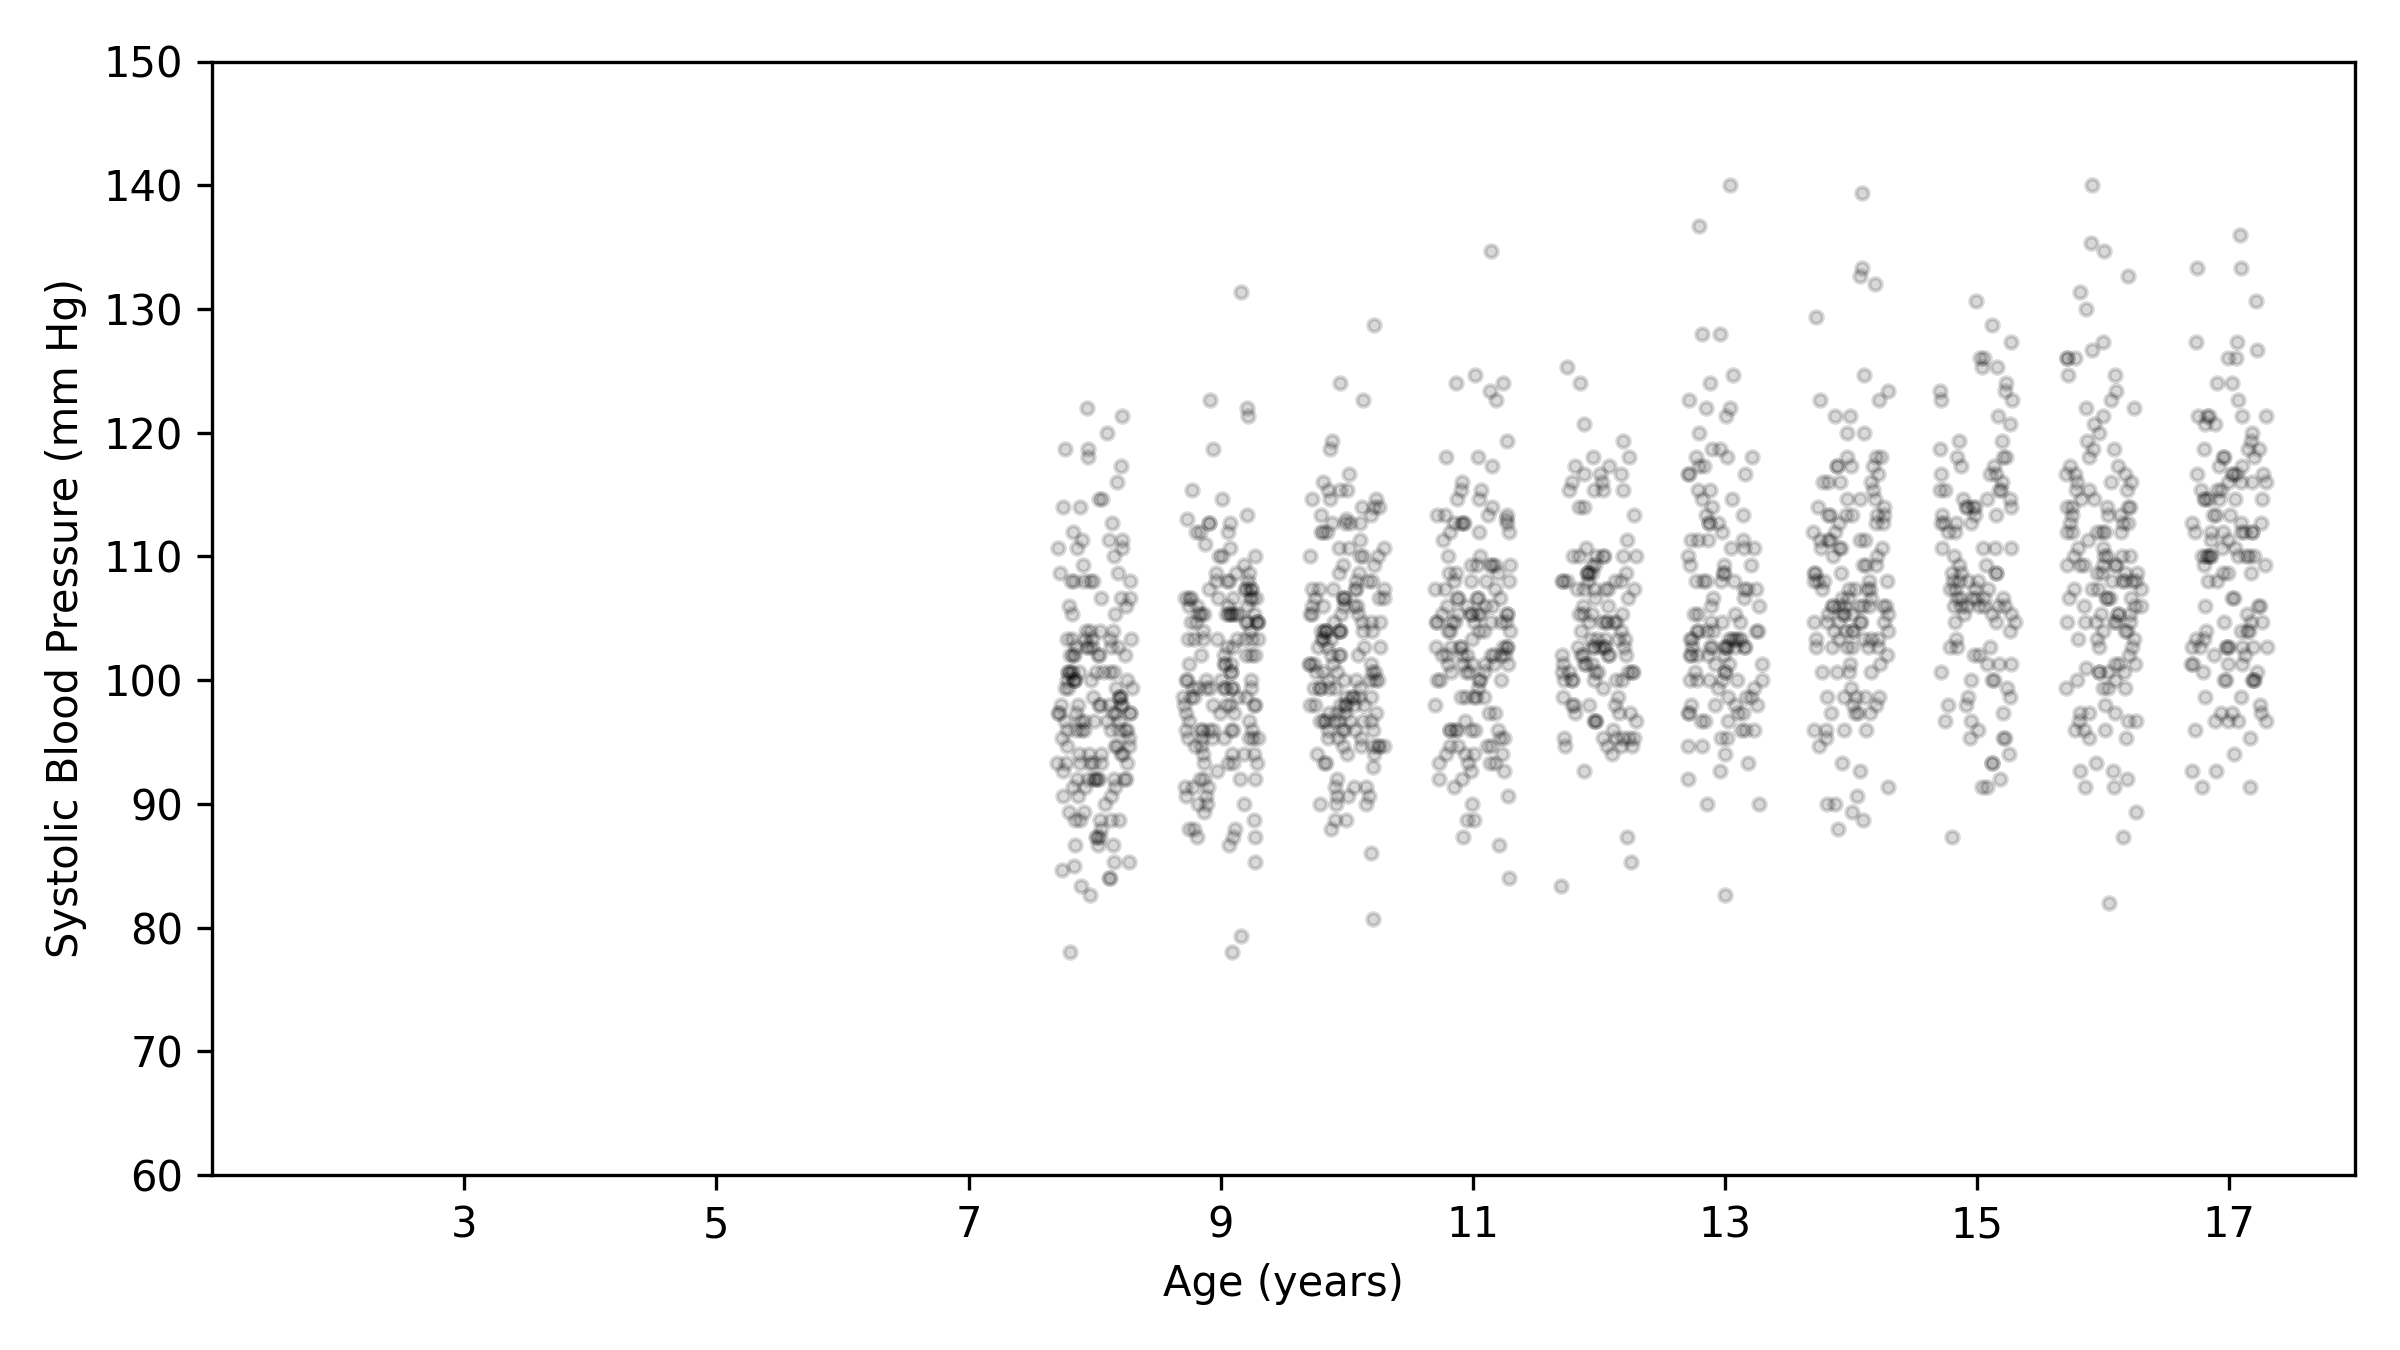
\includegraphics[width=0.92\linewidth]{images/missing_nhanes1.png}
	\end{center}
\end{frame}

\begin{frame}{Nonpositivity by Age in NHANES}
	In NHANES 2017-2018,
	\begin{itemize}
		\item ``BP is measured on participants 8 years and older"\footnote[frame]{\url{https://wwwn.cdc.gov/Nchs/Nhanes/2017-2018/BPX_J.htm}}
		\item $\Pr(R=1 \mid X=x) = 0$ for $x \in \{2,3,4,5,6,7\}$
	\end{itemize}
	~\\
	\begin{center}
		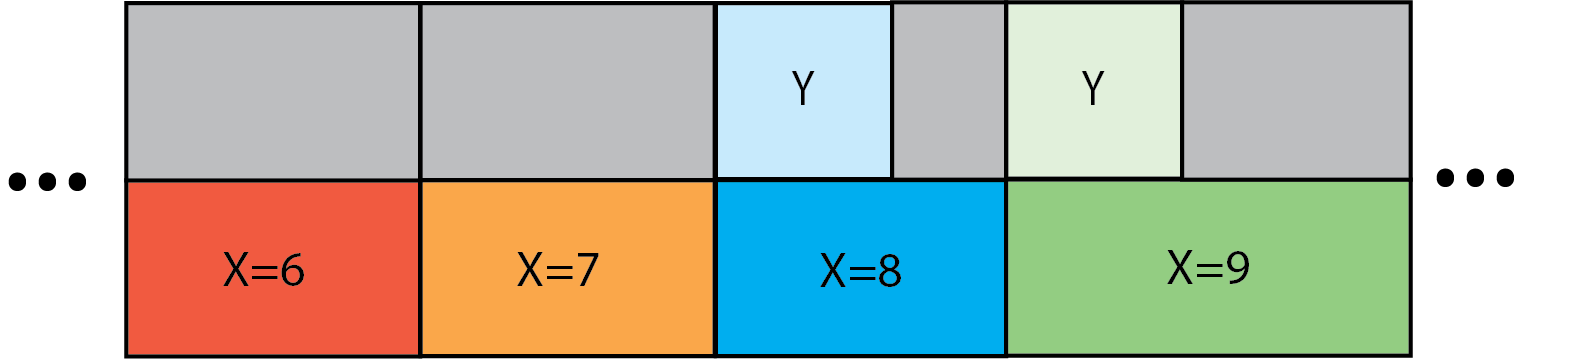
\includegraphics[width=0.85\linewidth]{images/missing-diagram2.png}
	\end{center}	
\end{frame}

\section{Addressing Positivity Violations}

\begin{frame}{Option 1: Change Parameter}
	\textbf{Parameter (revised)}: mean SBP {\color{darkred} for those 8 or older}
	$$ E[Y \mid X \ge 8] $$
	~\\
	\textbf{Question}: what is the mean systolic blood pressure (SBP) in mm Hg among children and adolescents {\color{darkred} aged 8-17} in the US?
	~\\~\\
	\begin{center}
		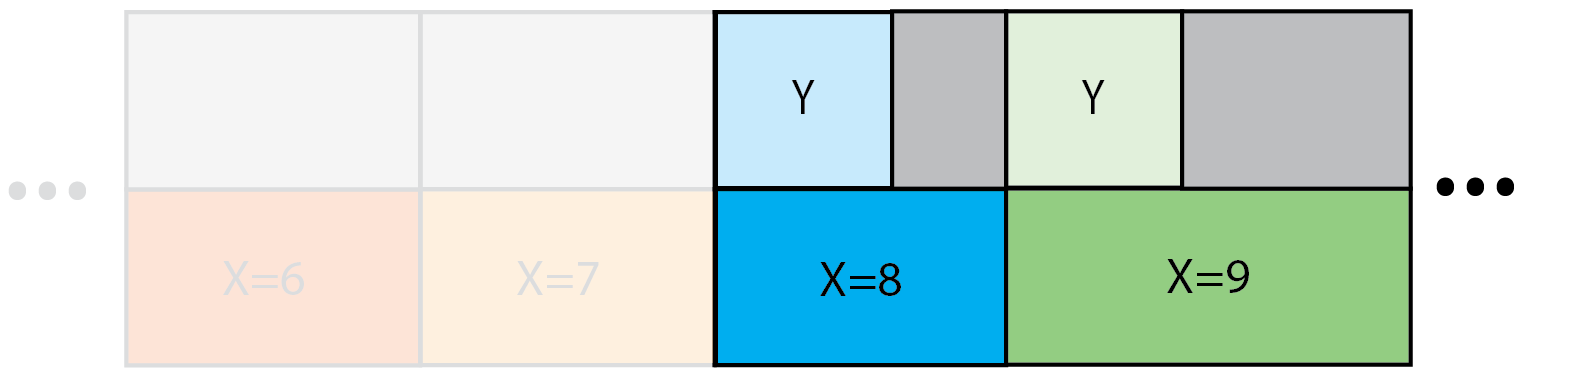
\includegraphics[width=0.7\linewidth]{images/missing-diagram3.png}
	\end{center}
\end{frame}

\begin{frame}{NHANES Data}
	\begin{center}
		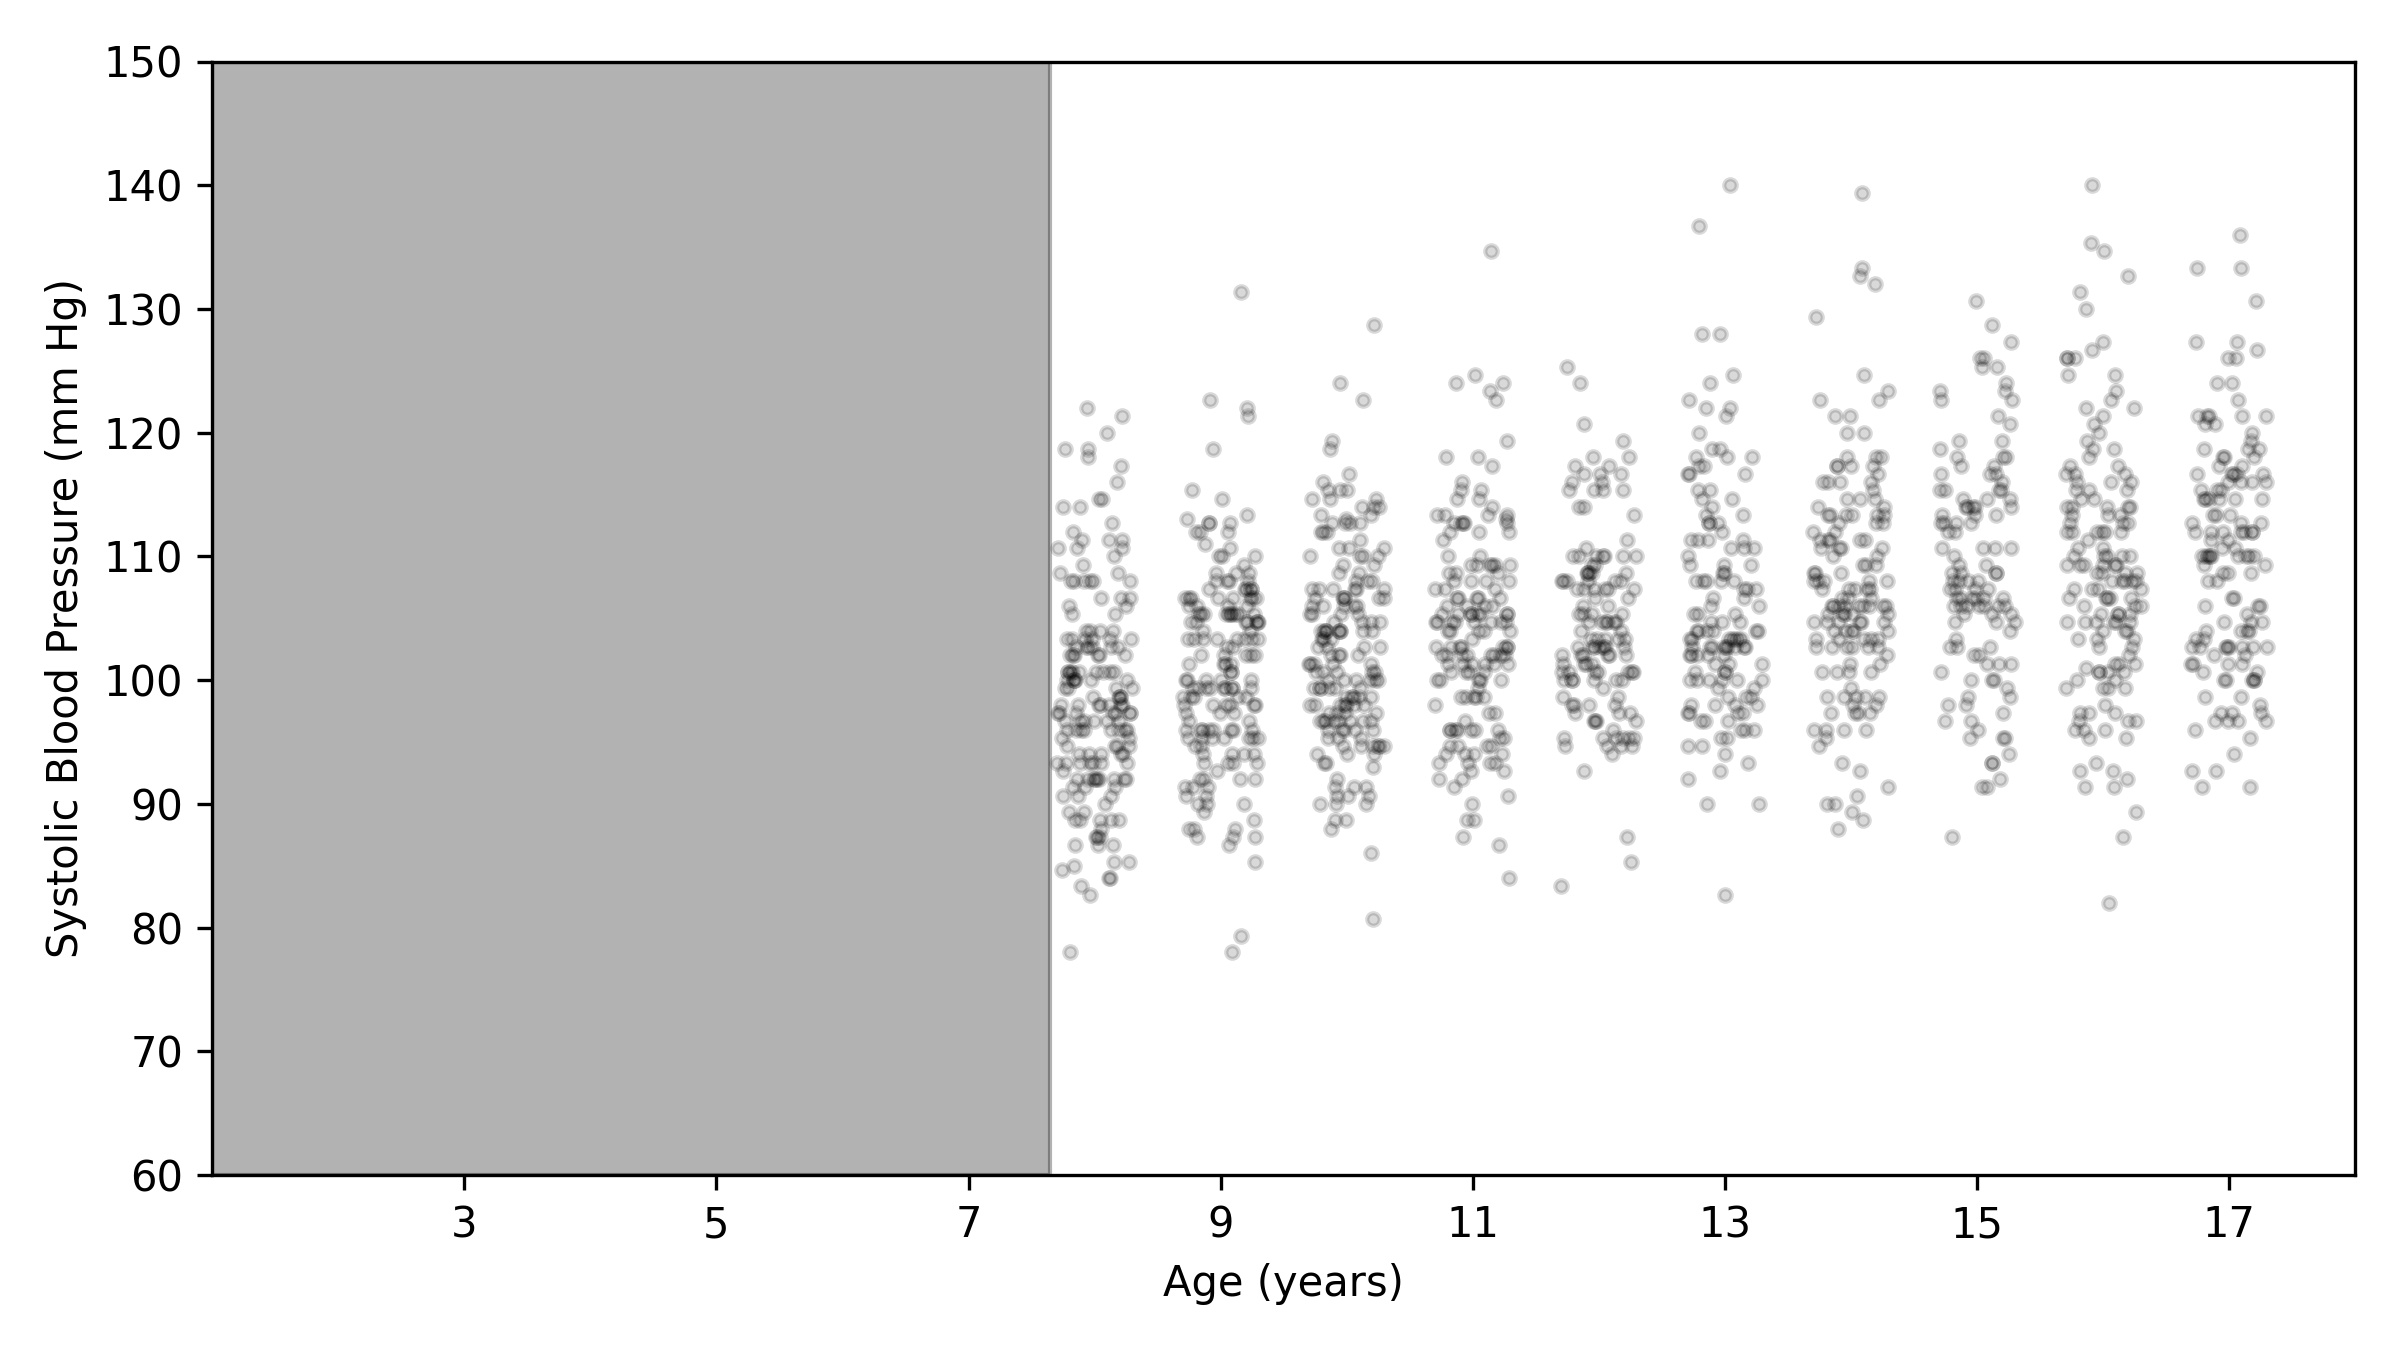
\includegraphics[width=0.92\linewidth]{images/missing_nhanes2.png}
	\end{center}
\end{frame}

\begin{frame}{Option 2. Extrapolate from Statistical Model}
	Fit a parametric model
	$$ E[Y \mid X \ge 8, R=1] = \beta_0 + \beta_1 X $$
	then fill in missing SBP with model predictions
	\begin{center}
		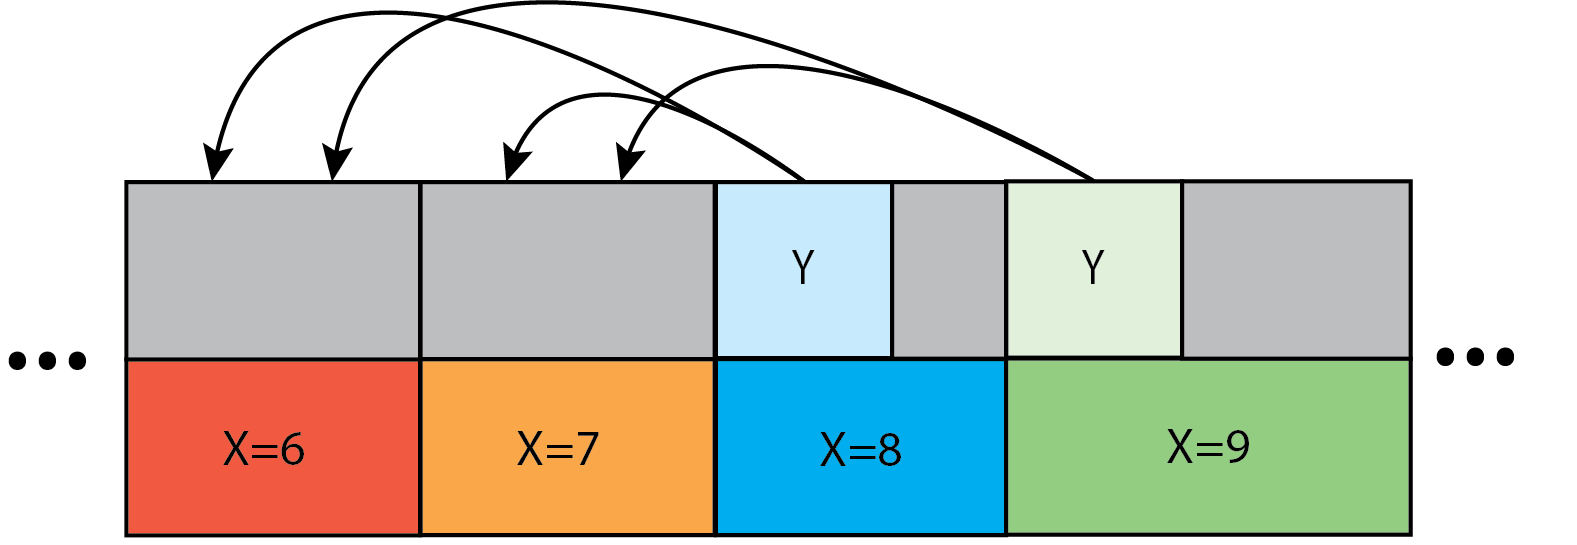
\includegraphics[width=0.7\linewidth]{images/missing-diagram4.png}
	\end{center}
\end{frame}

\begin{frame}{NHANES Data}
	\begin{center}
		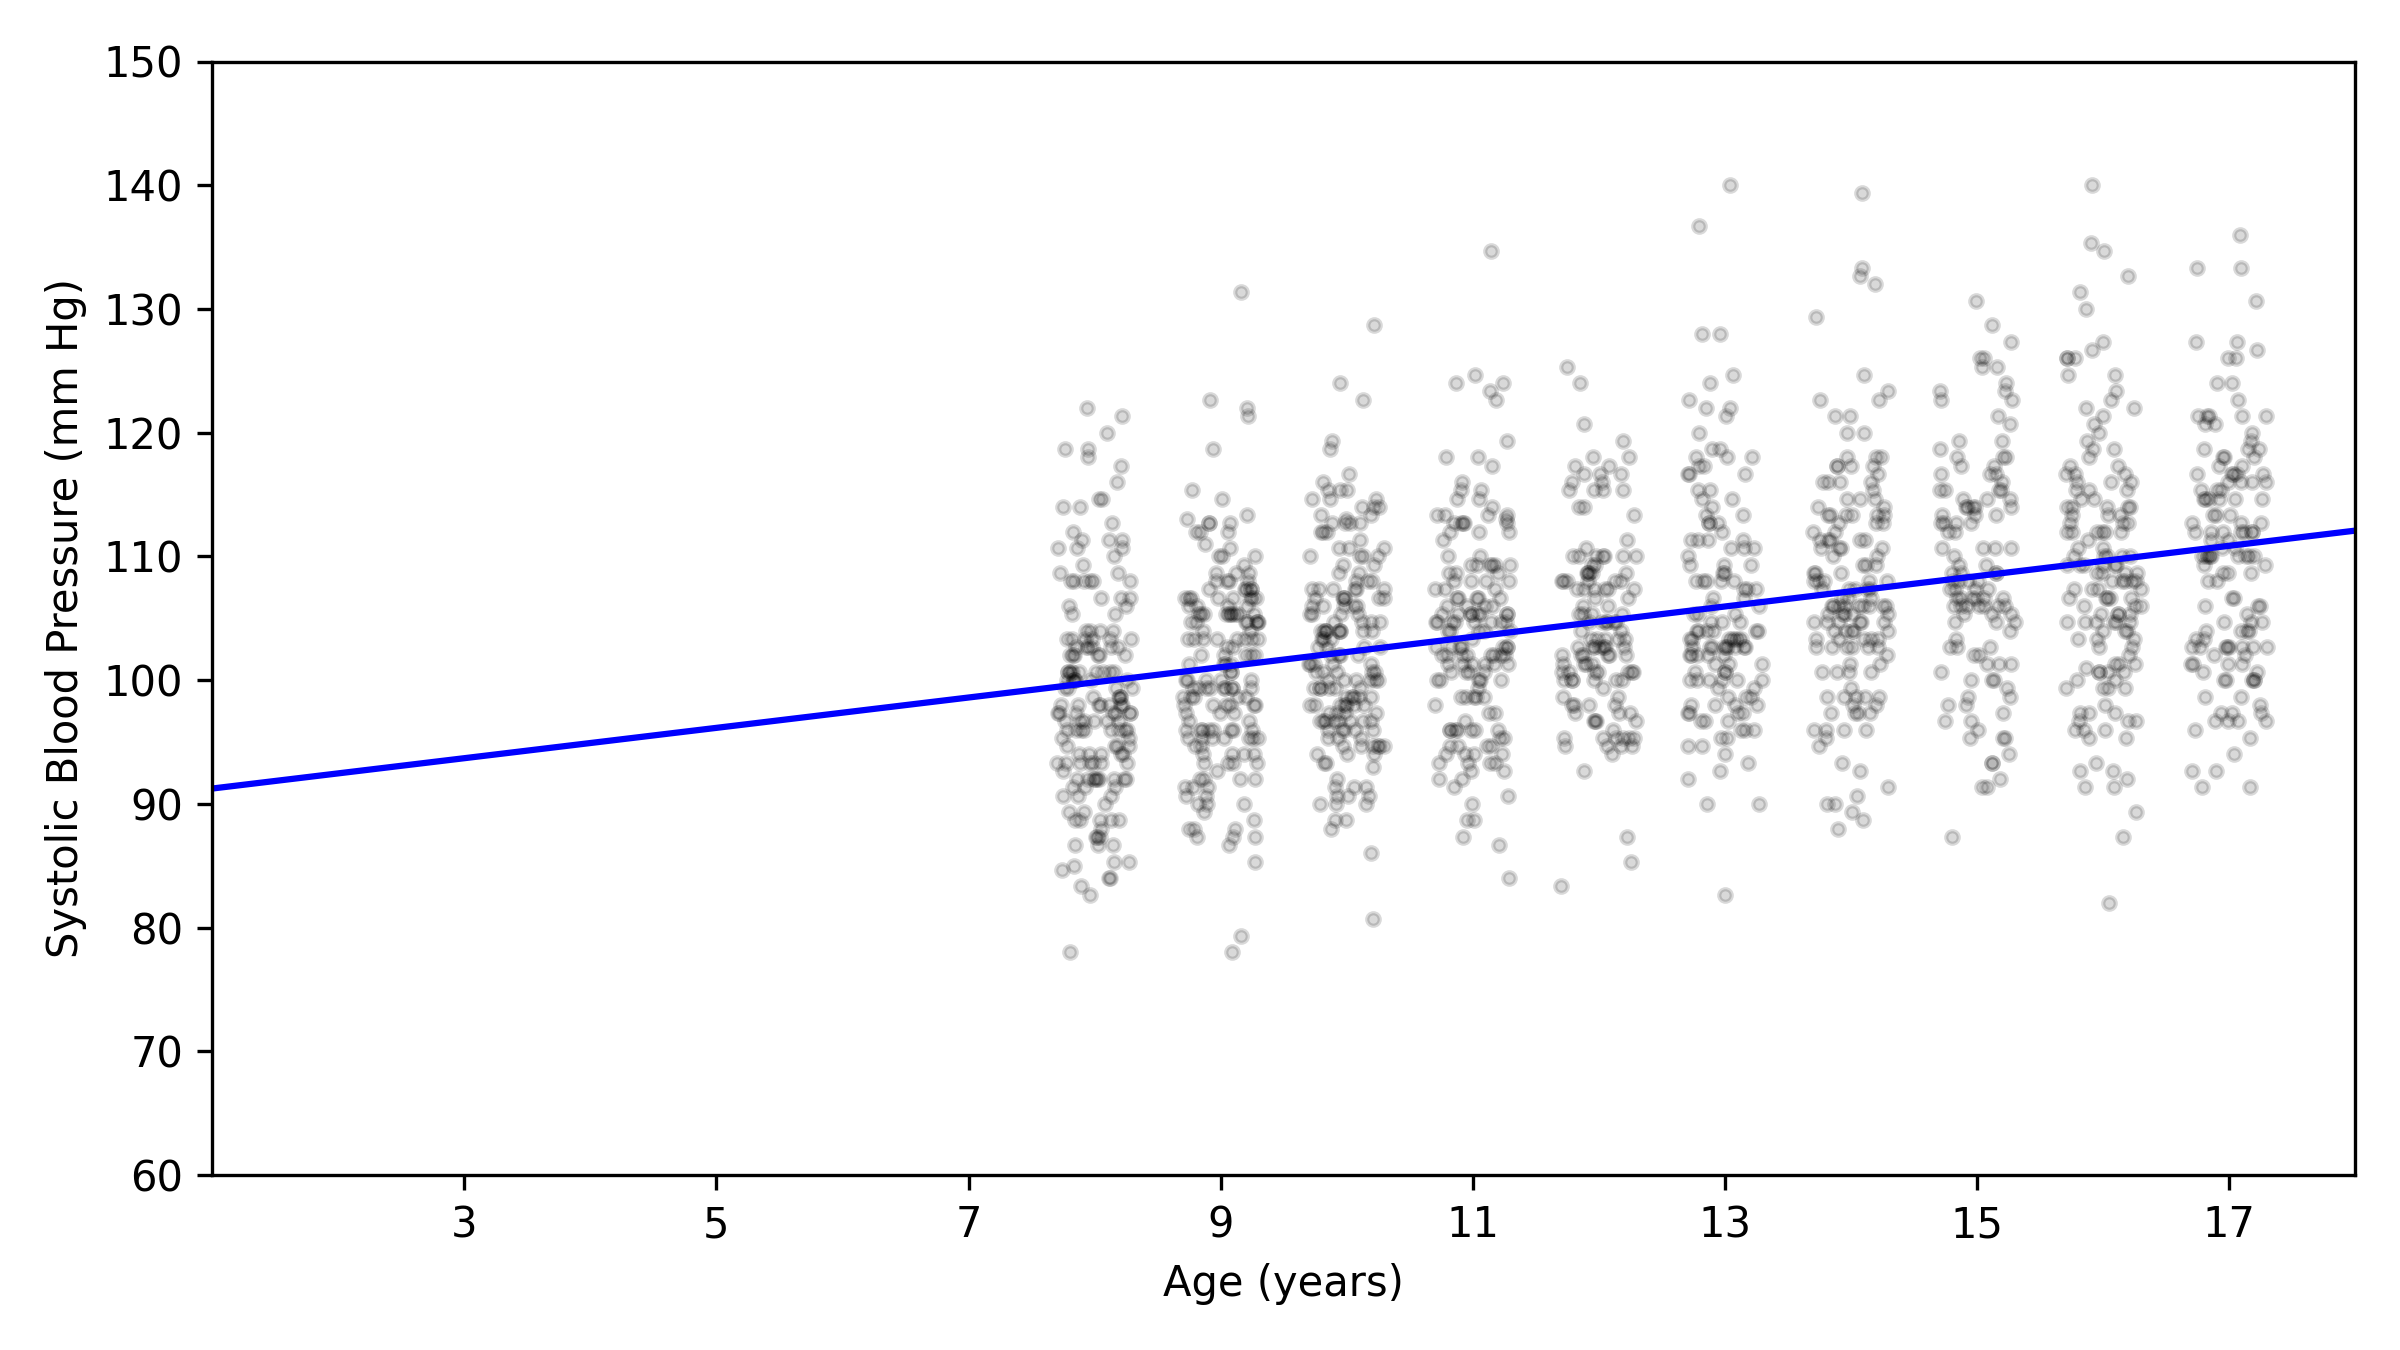
\includegraphics[width=0.92\linewidth]{images/missing_nhanes3.png}
	\end{center}
\end{frame}

\begin{frame}{NHANES Data}
	\begin{center}
		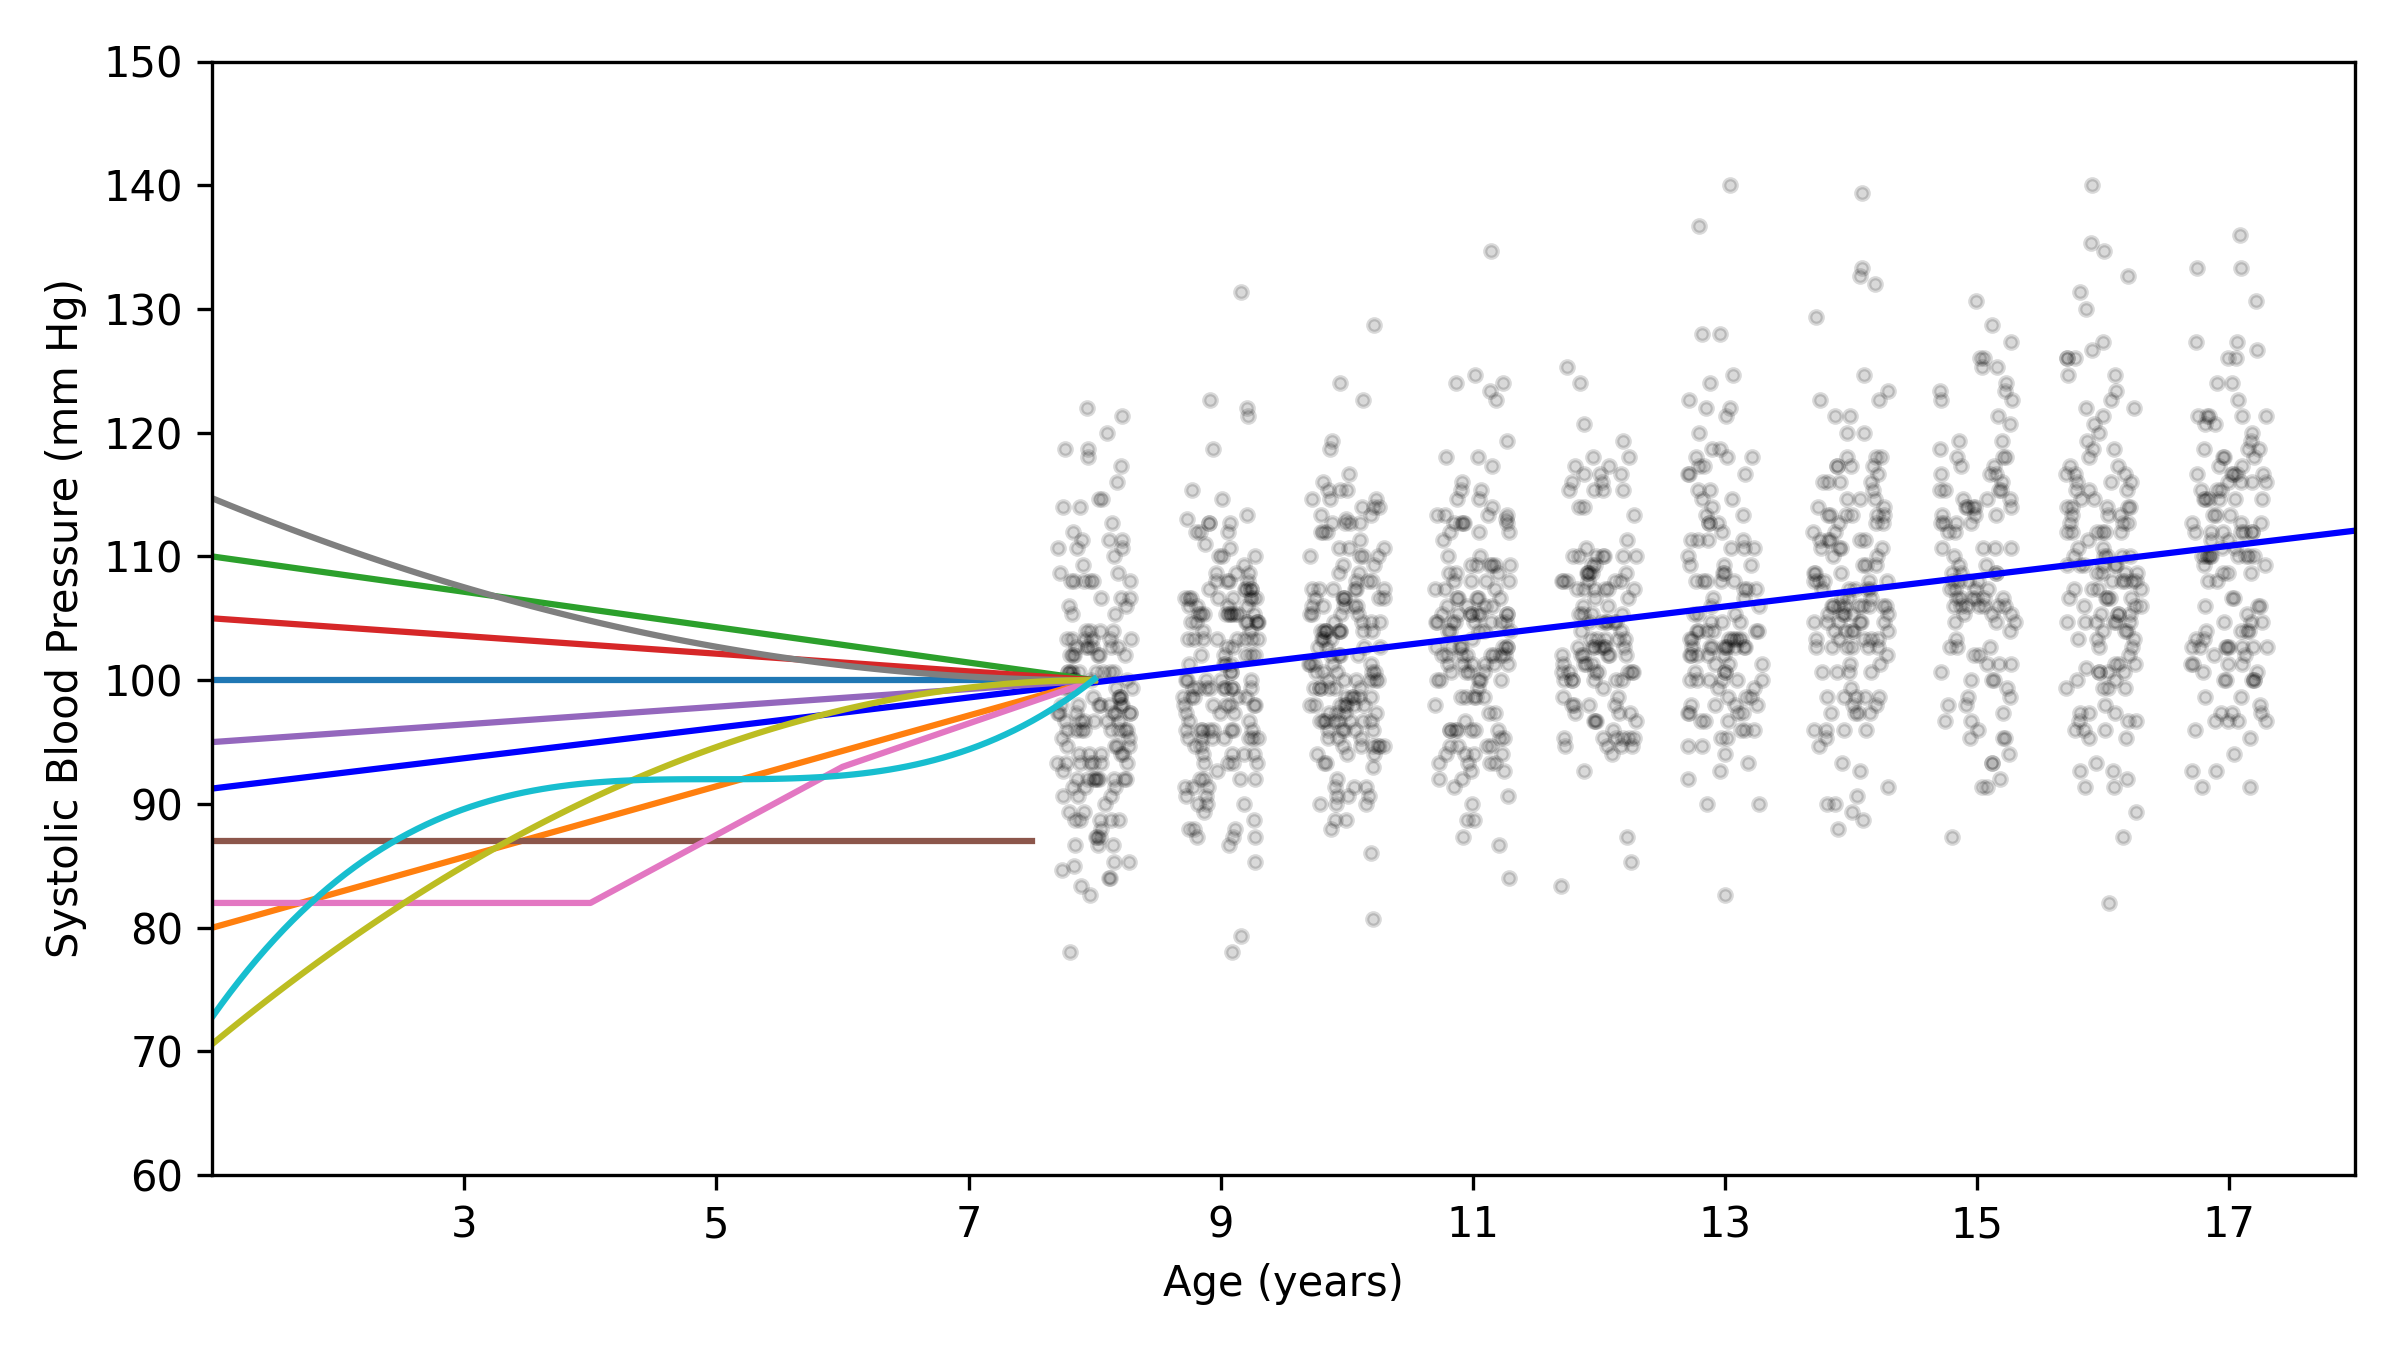
\includegraphics[width=0.92\linewidth]{images/missing_nhanes3b.png}
	\end{center}
\end{frame}

\begin{frame}{2. Extrapolate}
	Use of this model has two assumptions:
	\begin{itemize}
		\item[a.] Linear relationship with age for those 8-17 
		\item[b.] Linear relationship extends to those 2-7
	\end{itemize}
	~\\~\\
	(a) is in-principle checkable 
	\\~\\
	(b) is not checkable under nonpositivity
\end{frame}

\begin{frame}{Option 3: Bounds and Synthesis Modeling}
	Divide parameter of interest in parts
	\\~\\
	\begin{equation*}
		\eqnmarkbox[darkgreen]{node0}{\mu} = \eqnmarkbox[blue]{node1}{E[Y \mid X \ge 8]} \Pr(X \ge 8) + \eqnmarkbox[red]{node2}{E[Y \mid X < 8]} \Pr(X < 8)
	\end{equation*}
	\annotate[yshift=0.75em]{above,right}{node0}{Overall mean}	
	\annotate[yshift=-0.4em]{below,right}{node1}{Mean in positive region}	
	\annotate[yshift=0.75em]{above,left}{node2}{Mean in nonpositive region}	
	~\\~\\
	Here,
	$$ \eqnmarkbox[blue]{nodeZ}{E[Y \mid X \ge 8]} = E[E(Y \mid X, R=1, X \ge 8) \mid X \ge 8] $$
	from conditional exchangeability in positive region
\end{frame}

\begin{frame}{Option 3: Bounds and Synthesis Modeling}
	Available data leaves us stuck with $ \eqnmarkbox[red]{nodeZ}{E[Y \mid X < 8]} = \; ?$
	~\\~\\
	To progress, will appeal to external information for
	\begin{itemize}
		\item[a.] Bounds
		\item[b.] Sensitivity Analysis
		\item[c.] Point Identification
	\end{itemize}
	\begin{center}
		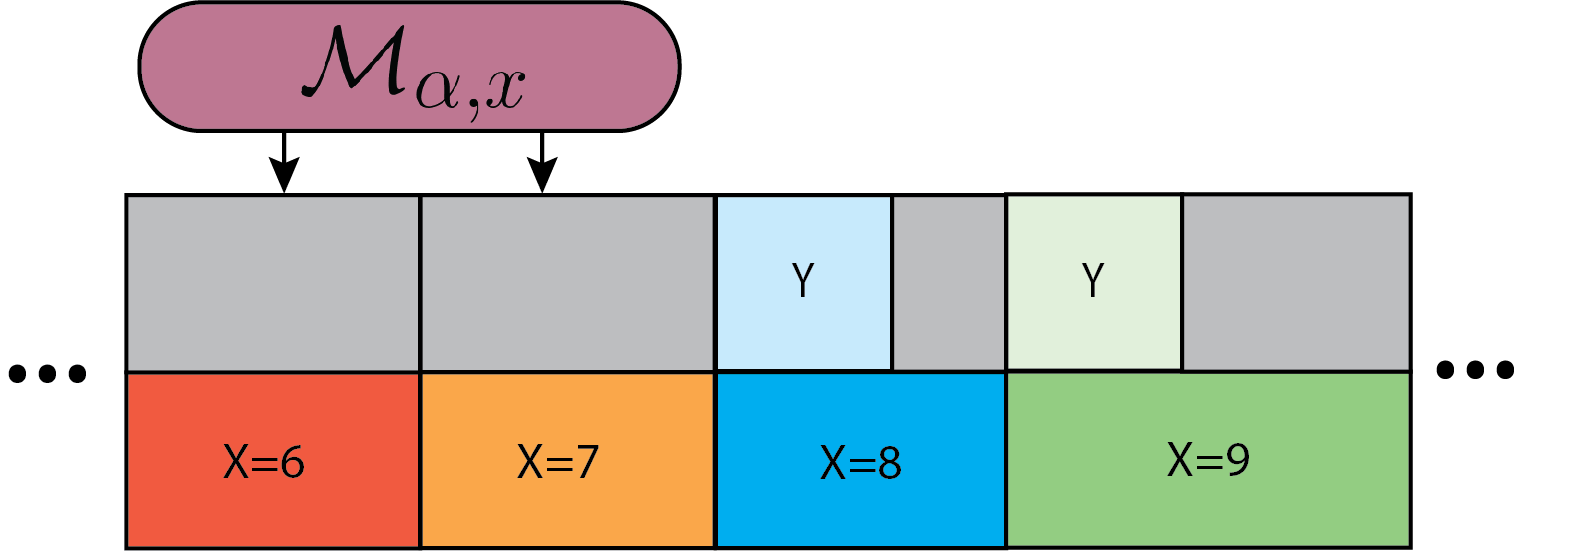
\includegraphics[width=0.7\linewidth]{images/missing-diagram5.png}
	\end{center}
\end{frame}

\begin{frame}{Option 3a: Bounds}
	In our context, know that SBP must be a (finite) positive number, so
	$$ E[Y \mid X=x] \in (0, \infty) \text{ for all } x \in \{2, 3, 4, 5, 6, 7\}$$
	~\\
	Context allows us to further narrow the plausible region to
	$$ E[Y \mid X=x] \in [140, 200] \text{ for all } x \in \{2, 3, 4, 5, 6, 7\}$$
	as these boundary values would constitute medical emergencies
	~\\~\\
	Therefore, 
	$$ 50 + \Pr(X \ge 8)\left\{\eqnmarkbox[blue]{nodeZ1}{E[Y \mid X \ge 8]} - 50\right\} \le \eqnmarkbox[darkgreen]{nodeZ0}{\mu} \le 200 + \Pr(X \ge 8)\left\{\eqnmarkbox[blue]{nodeZ2}{E[Y \mid X \ge 8]} - 200\right\}$$ 
\end{frame}

\begin{frame}{Option 3b: Sensitivity Analysis}
	Rather than evaluate at the extremes, evaluate
	\begin{equation*}
		\eqnmarkbox[darkgreen]{node0}{\mu} = \eqnmarkbox[blue]{node1}{E[E(Y \mid X, R=1, X \ge 8) \mid X \ge 8]} \Pr(X \ge 8) + \eqnmarkbox[red]{node2}{q} \Pr(X < 8)
	\end{equation*}
	where $q \in [50, 200]$
	~\\~\\~\\
	Assess how $\mu$ varies as a function of the possible means for the nonpositive region 
	\begin{itemize}
		\item May help to further contextualize the bounds
	\end{itemize}
\end{frame}

\begin{frame}{Option 3c: Leverage a Mathematical Model}
	Previous only provide range of equally plausible values
	\begin{itemize}
		\item Can leverage more specific information when available
		\item Published distributions of SBP by age, gender, height\footnote[frame]{Flynn et al. 2017 \textit{Pediatrics} 140(3):e20171904}
	\end{itemize}
	~\\~\\
	Use this additional information to construct a mathematical model that produces a probability distribution $\mathcal{M}_{\alpha,x}$ for age $x$ given parameters $\alpha$, and assume
	$$ E[Y \mid X=x] \in \mathcal{M}_{\alpha,x} \text{ for all } x \in \{2, 3, 4, 5, 6, 7\}$$
\end{frame}

\begin{frame}{Option 3c: Synthesis of Statistical and Mathematical Models}
	Then can combine statistical and mathematical models for identification
	\begin{equation*}
		\begin{aligned}
			\eqnmarkbox[darkgreen]{node0}{\mu} = & \eqnmarkbox[blue]{node1}{E[E(Y \mid X, R=1, X \ge 8) \mid X \ge 8]} \Pr(X \ge 8) \\
			& + \eqnmarkbox[red]{node2}{E[E(\mathcal{M}_{\alpha,x} \mid X, X<8) \mid X<8]} \Pr(X < 8)
		\end{aligned}
	\end{equation*}
	~\\~\\~\\
	Build $\mathcal{M}_{\alpha,x}$ from published age-, gender-, and height-specific SBP distributions
\end{frame}

\begin{frame}{NHANES Data}
	\begin{center}
		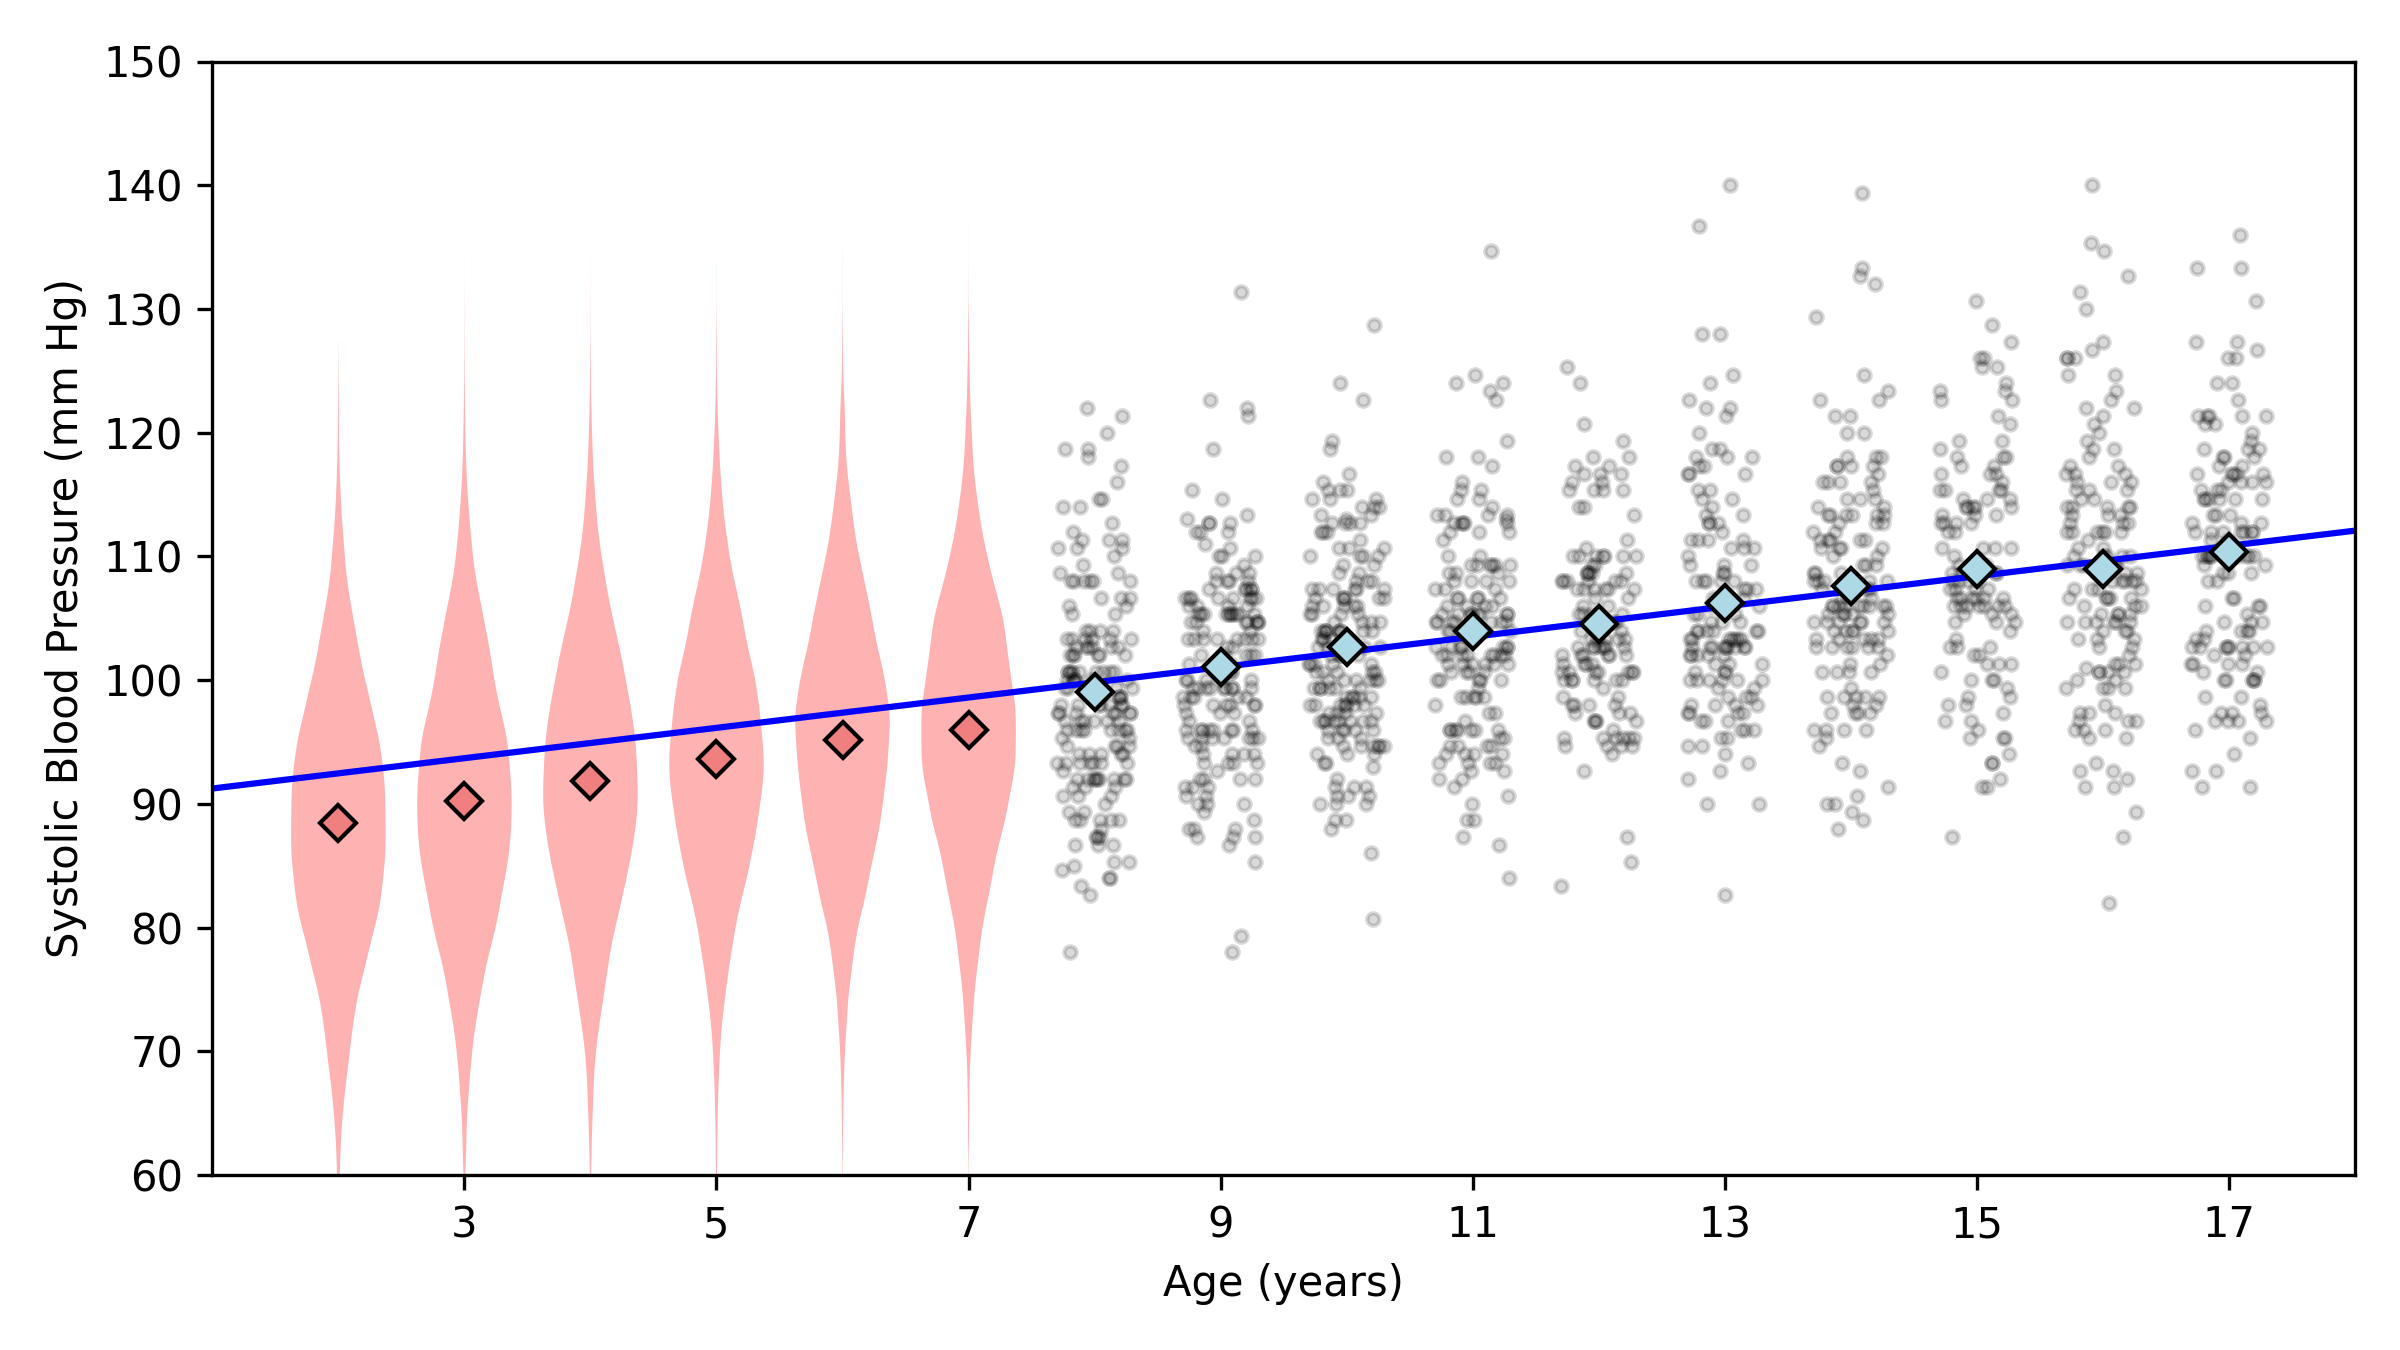
\includegraphics[width=0.92\linewidth]{images/missing_nhanes4.png}
	\end{center}
\end{frame}

\begin{frame}{Estimators for Option 3}
	\textbf{Option 3a/b}: estimate $E[E(Y \mid X,R=1,X \ge 8) \mid X \ge 8]$ using statistical modeling, \footnote[frame]{Here, I use g-computation for ease but could also use IPW or AIPW. The publication applies all three} set $q$, solve for $\mu$.\footnote[frame]{Use the pointwise Confidence Intervals which are conservative, Richardson et al. \textit{Stat Sci} 2014;29(4):596-618}
	~\\~\\
	\textbf{Option 3c}: Monte Carlo procedure to capture uncertainty
	\begin{itemize}
		\item[1.] Resample with replacement observed data 
		\item[2.] Estimate a statistical model for $E(Y \mid X,R=1,X \ge 8)$ and then impute $Y$ for observations with $X \ge 8$
		\item[3.] For those $X < 8$, impute $Y$ using a random draw from the mathematical model covariate-specific distributions
		\item[4.] Take the mean of the imputed $Y$ for all observations
	\end{itemize}
\end{frame}

\begin{frame}{Results by Method}
	\begin{center}
		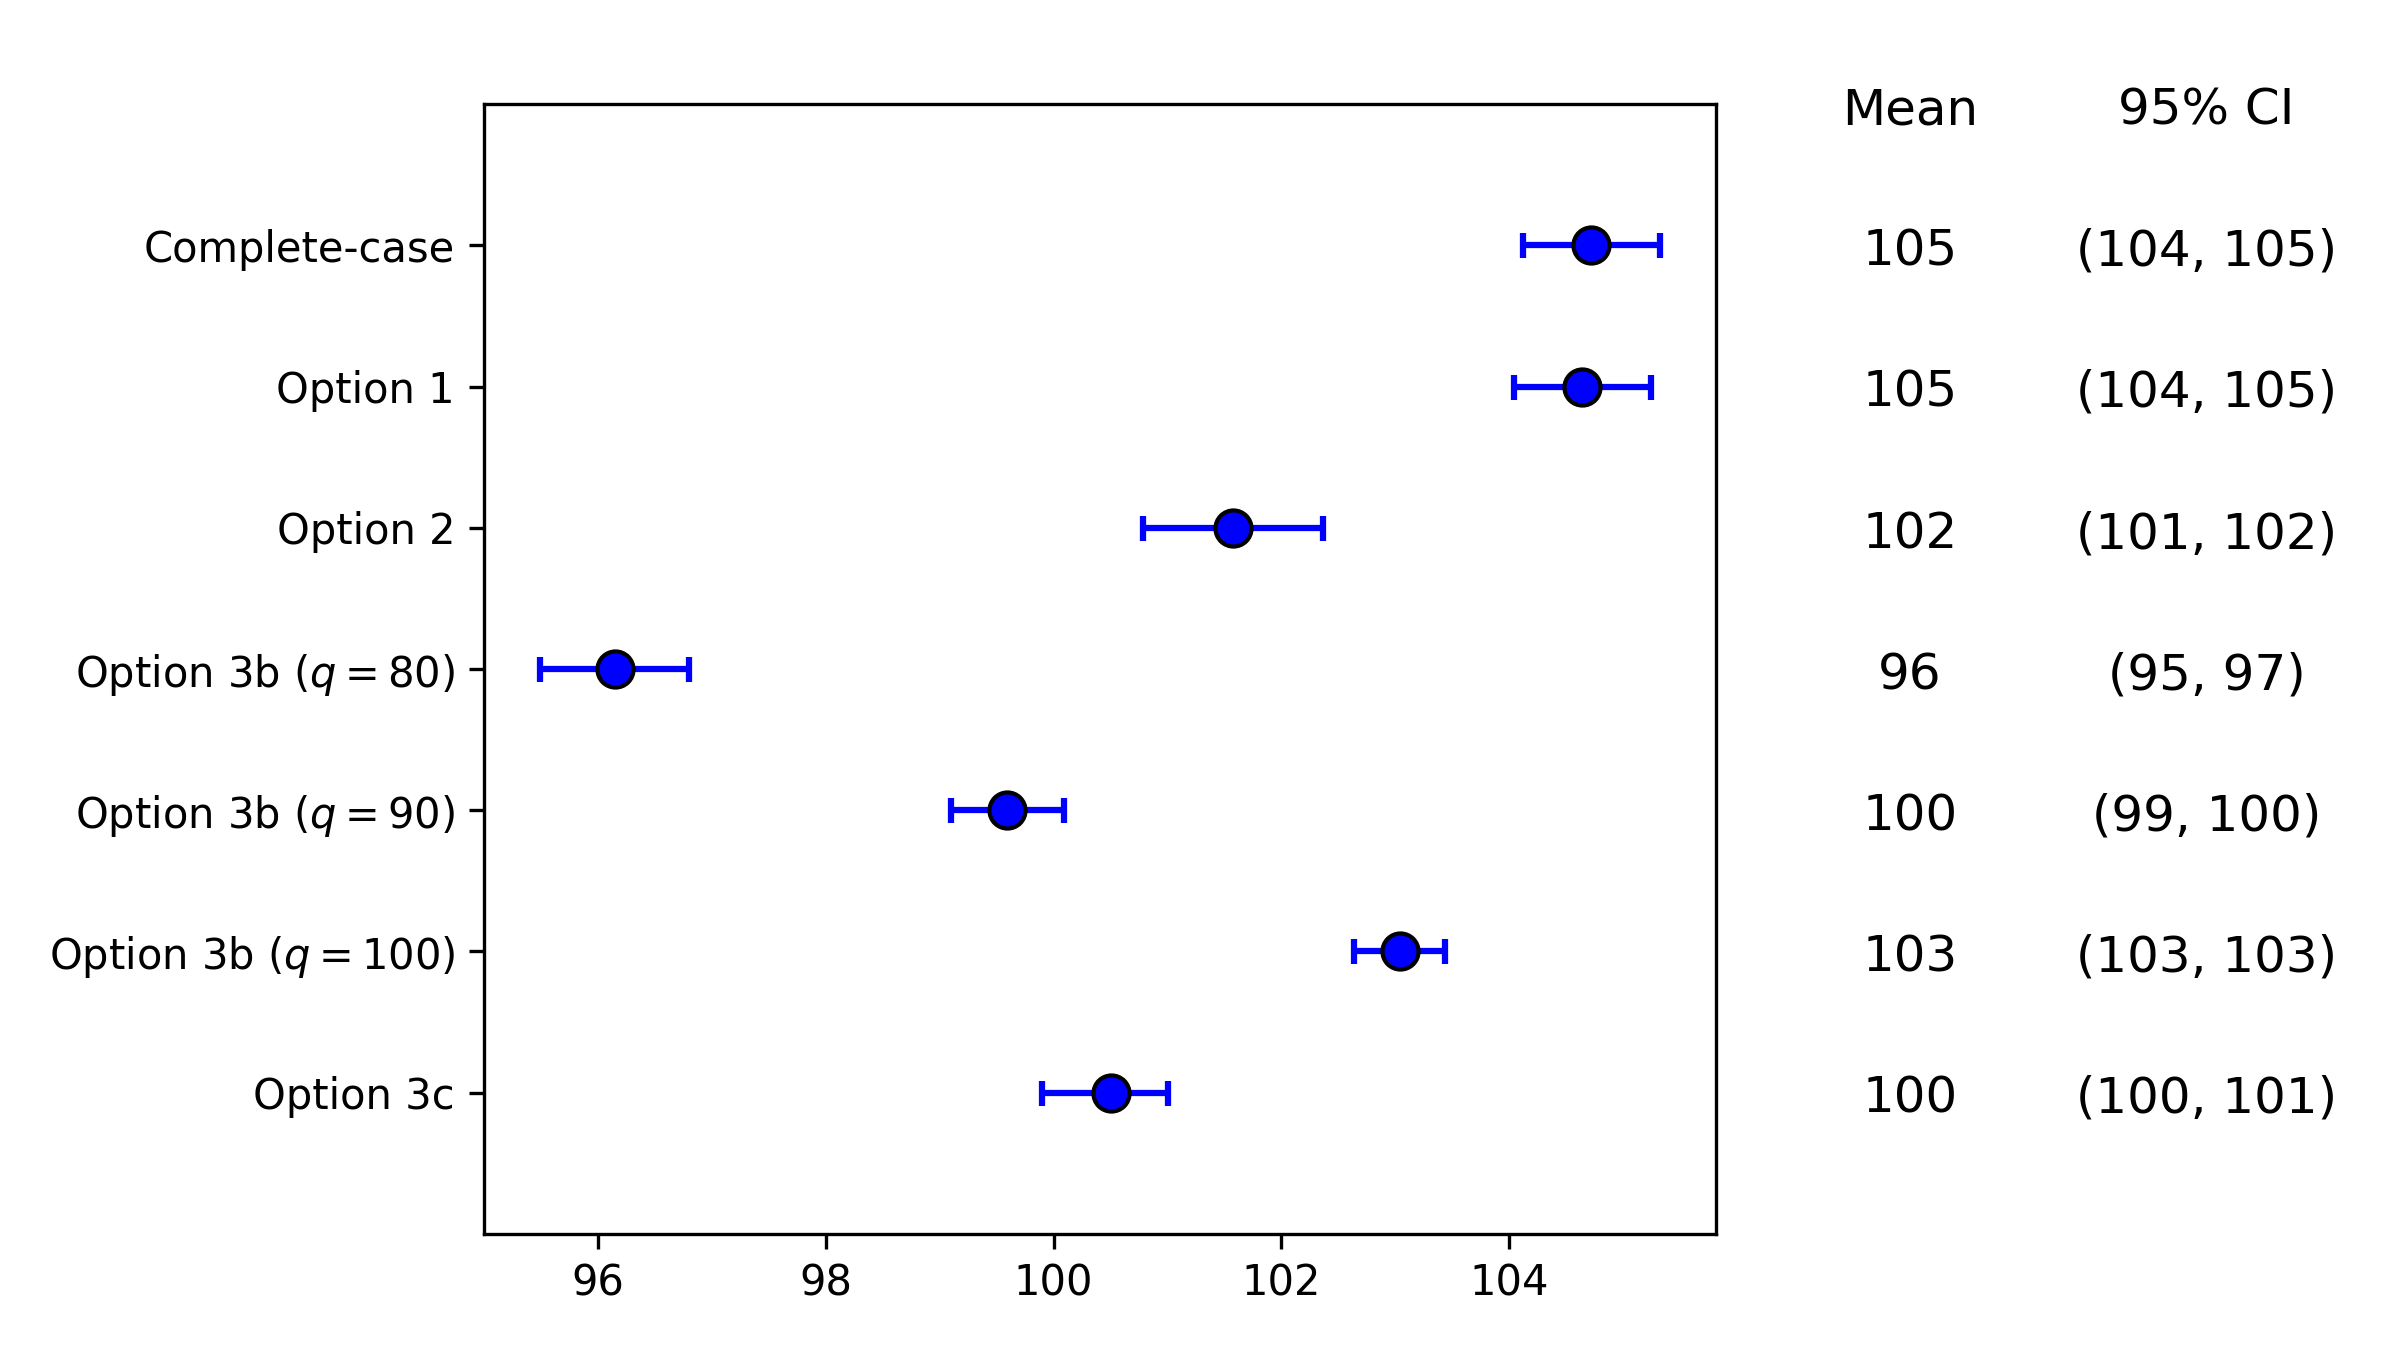
\includegraphics[width=0.92\linewidth]{images/results_acic.png}
	\end{center}
\end{frame}

\section{Conclusions}

\begin{frame}{Summary}
	Positivity is often neglected as an assumption
	\begin{itemize}
		\item But it remains vital for identification of many parameters
	\end{itemize}
	~\\
	Restricting parameters to positive regions often reasonable
	\begin{itemize}
		\item But may limit utility of research
		\item Extrapolation premised on strong assumptions
		\item Synthesis modeling allows for exploration and weakening of extrapolation assumptions
	\end{itemize}
\end{frame}

\begin{frame}{Future Directions}
	Compare statistical and mathematical models for positive region
	\begin{itemize}
		\item May provide some assurance for mathematical model
		\item Regularize statistical model for efficiency
	\end{itemize}
	~\\
	Exchangeability (and thus positivity) is used to address other systematic errors
	\begin{itemize}
		\item Approach can be used to address nonpositivity in these settings\footnote[frame]{Originally proposed in the context of transporting trials: Zivich et al. \textit{Epidemiology} 2024;35(1):23-31, Zivich et al. \textit{JRSSA} 2025;188(1):158-180}
	\end{itemize}
	~\\
	Analysis of mathematical models and improving their robustness\footnote[frame]{Some work on formalizing identification with mathematical models: Zivich \textit{arXiv:2511.01960}}
\end{frame}

\begin{frame}{Thank You!}
	\textbf{Publication}: Zivich et al. \textit{J Epidemiol Community Health} 2026;80:352-356
	~\\~\\~\\~\\
	\begin{center}
		\small
		\faEnvelope \quad pzivich@unc.edu \qquad \quad 
		\faGithub \quad pzivich \qquad \quad
		\faHashtag \quad pausalz@bsky.social
	\end{center}	
\end{frame}

\section{Appendix}

\begin{frame}{Comparing Statistical and Mathematical Models}
	\begin{center}
		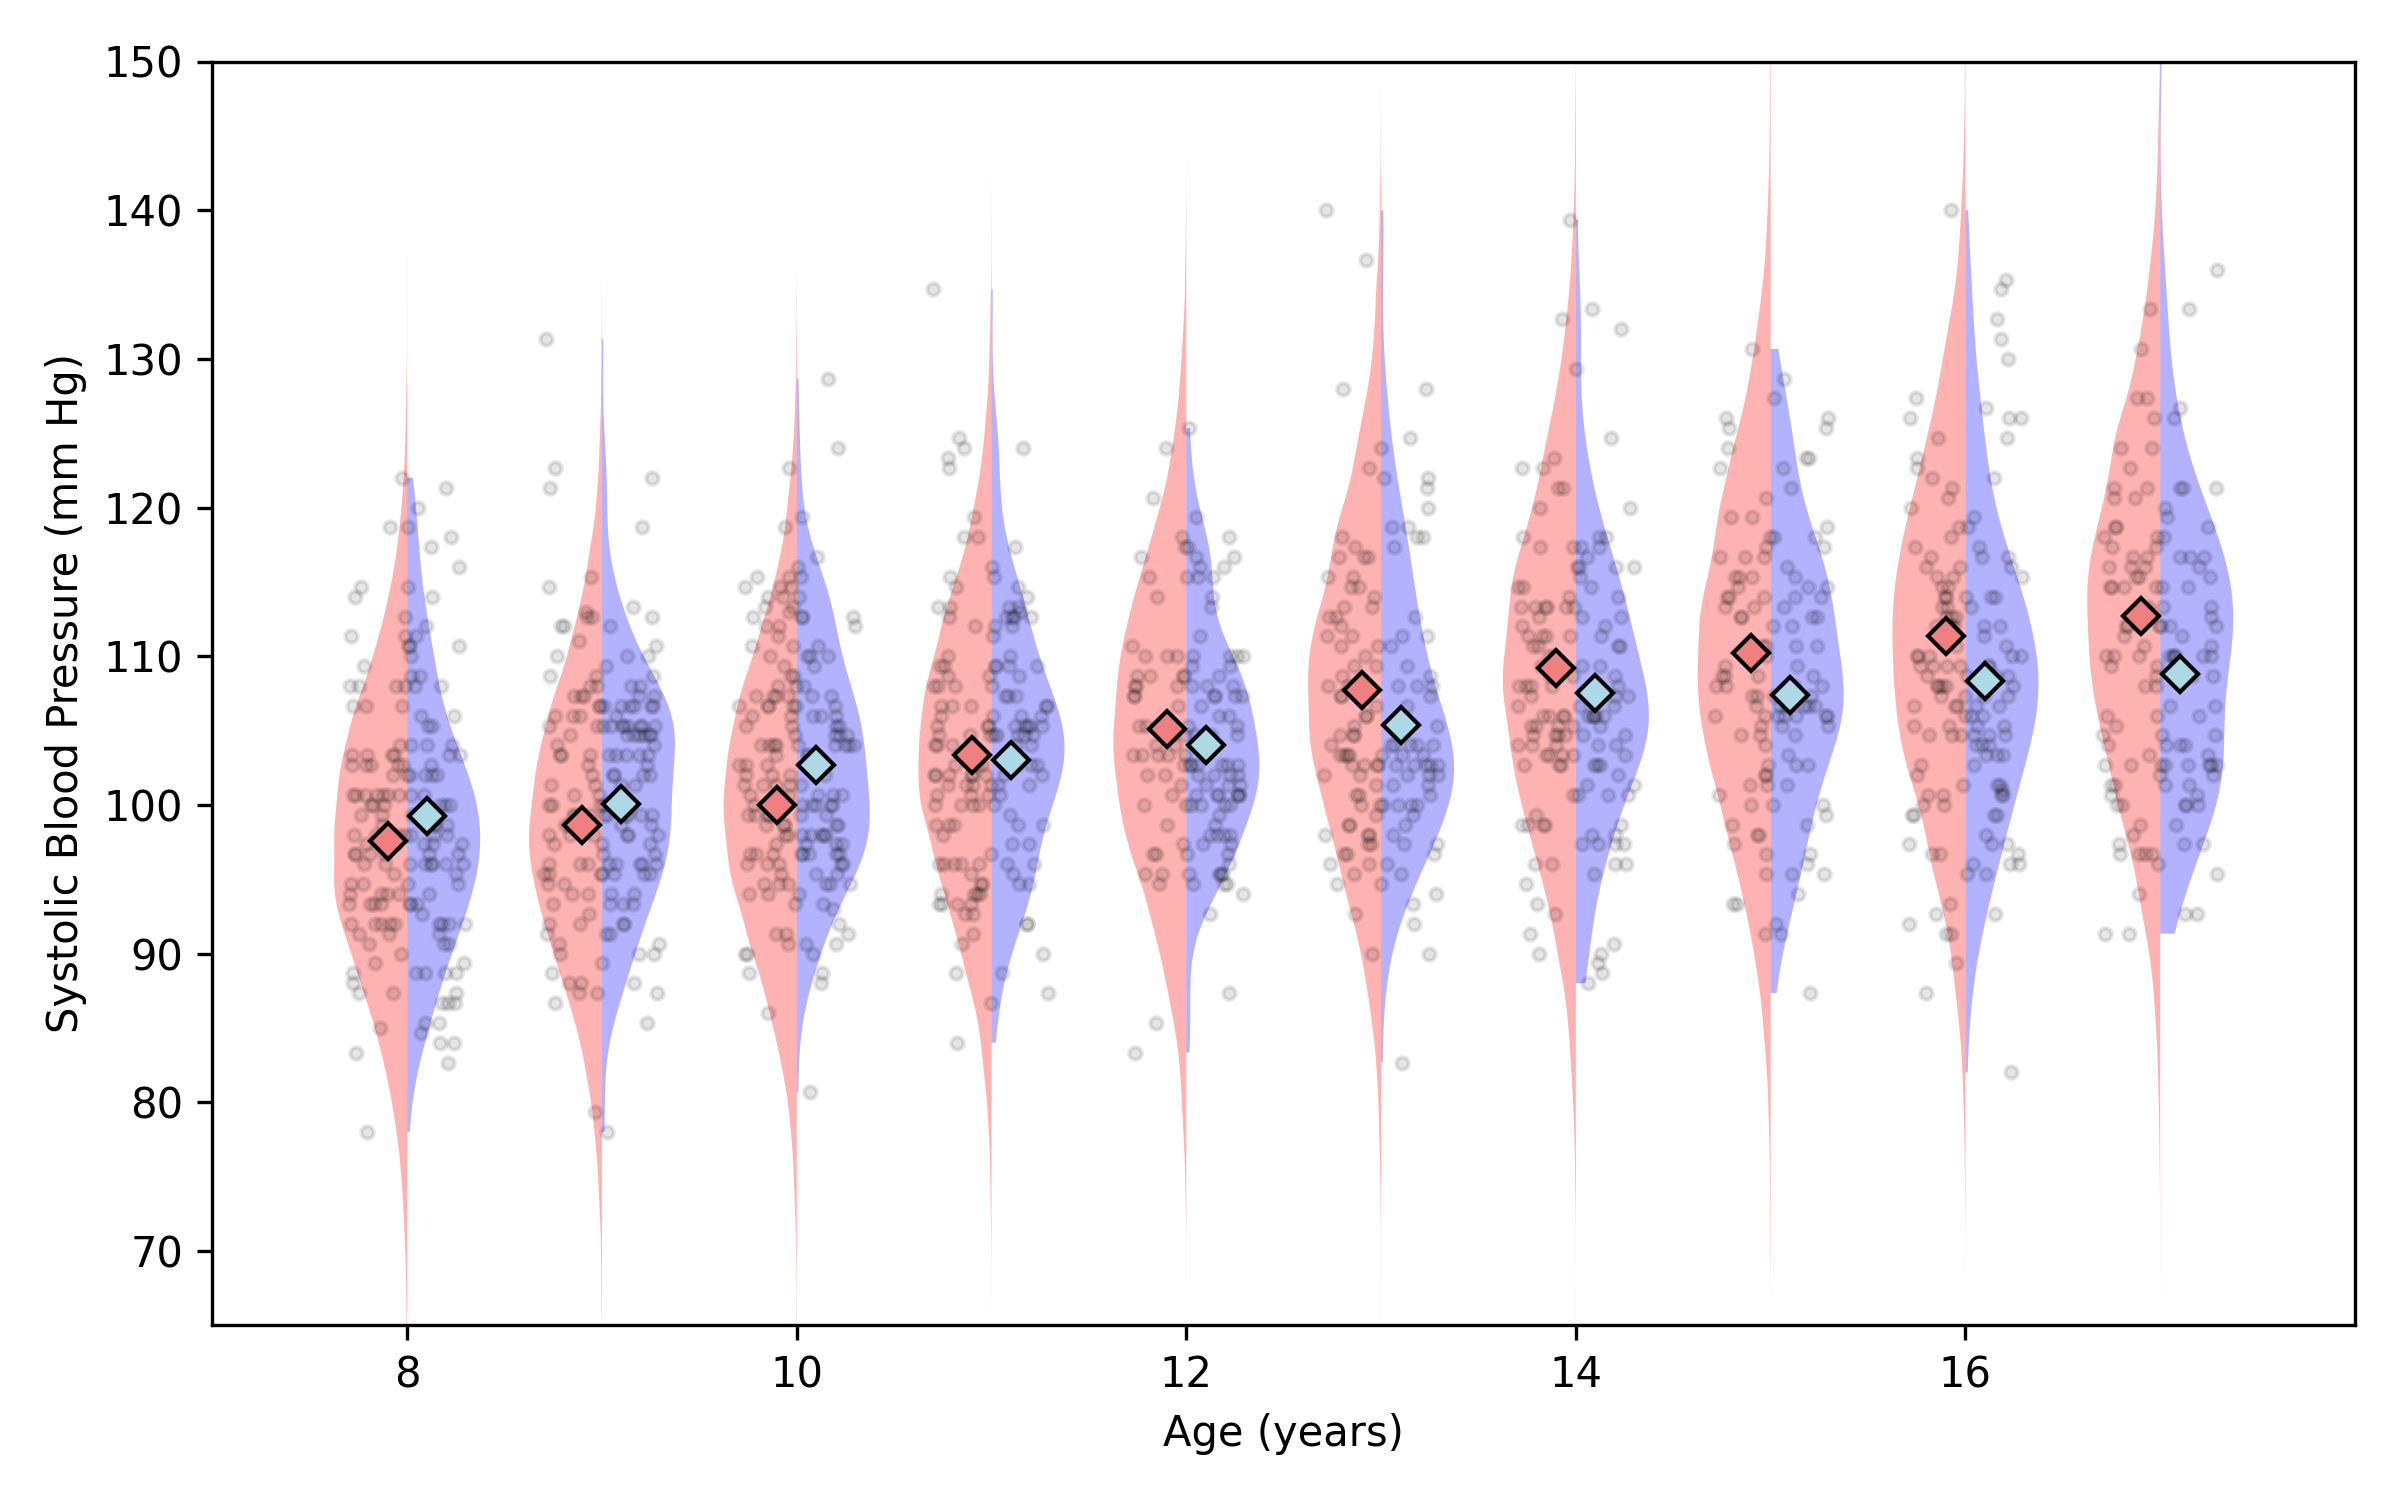
\includegraphics[width=0.85\linewidth]{images/diagnostic_plot1.png}
	\end{center}
\end{frame}

\begin{frame}{Comparing Statistical and Mathematical Models\footnote[frame]{Intervals are pointwise 95\% confidence intervals, so anti-conservative for overall comparison}}
	\begin{center}
		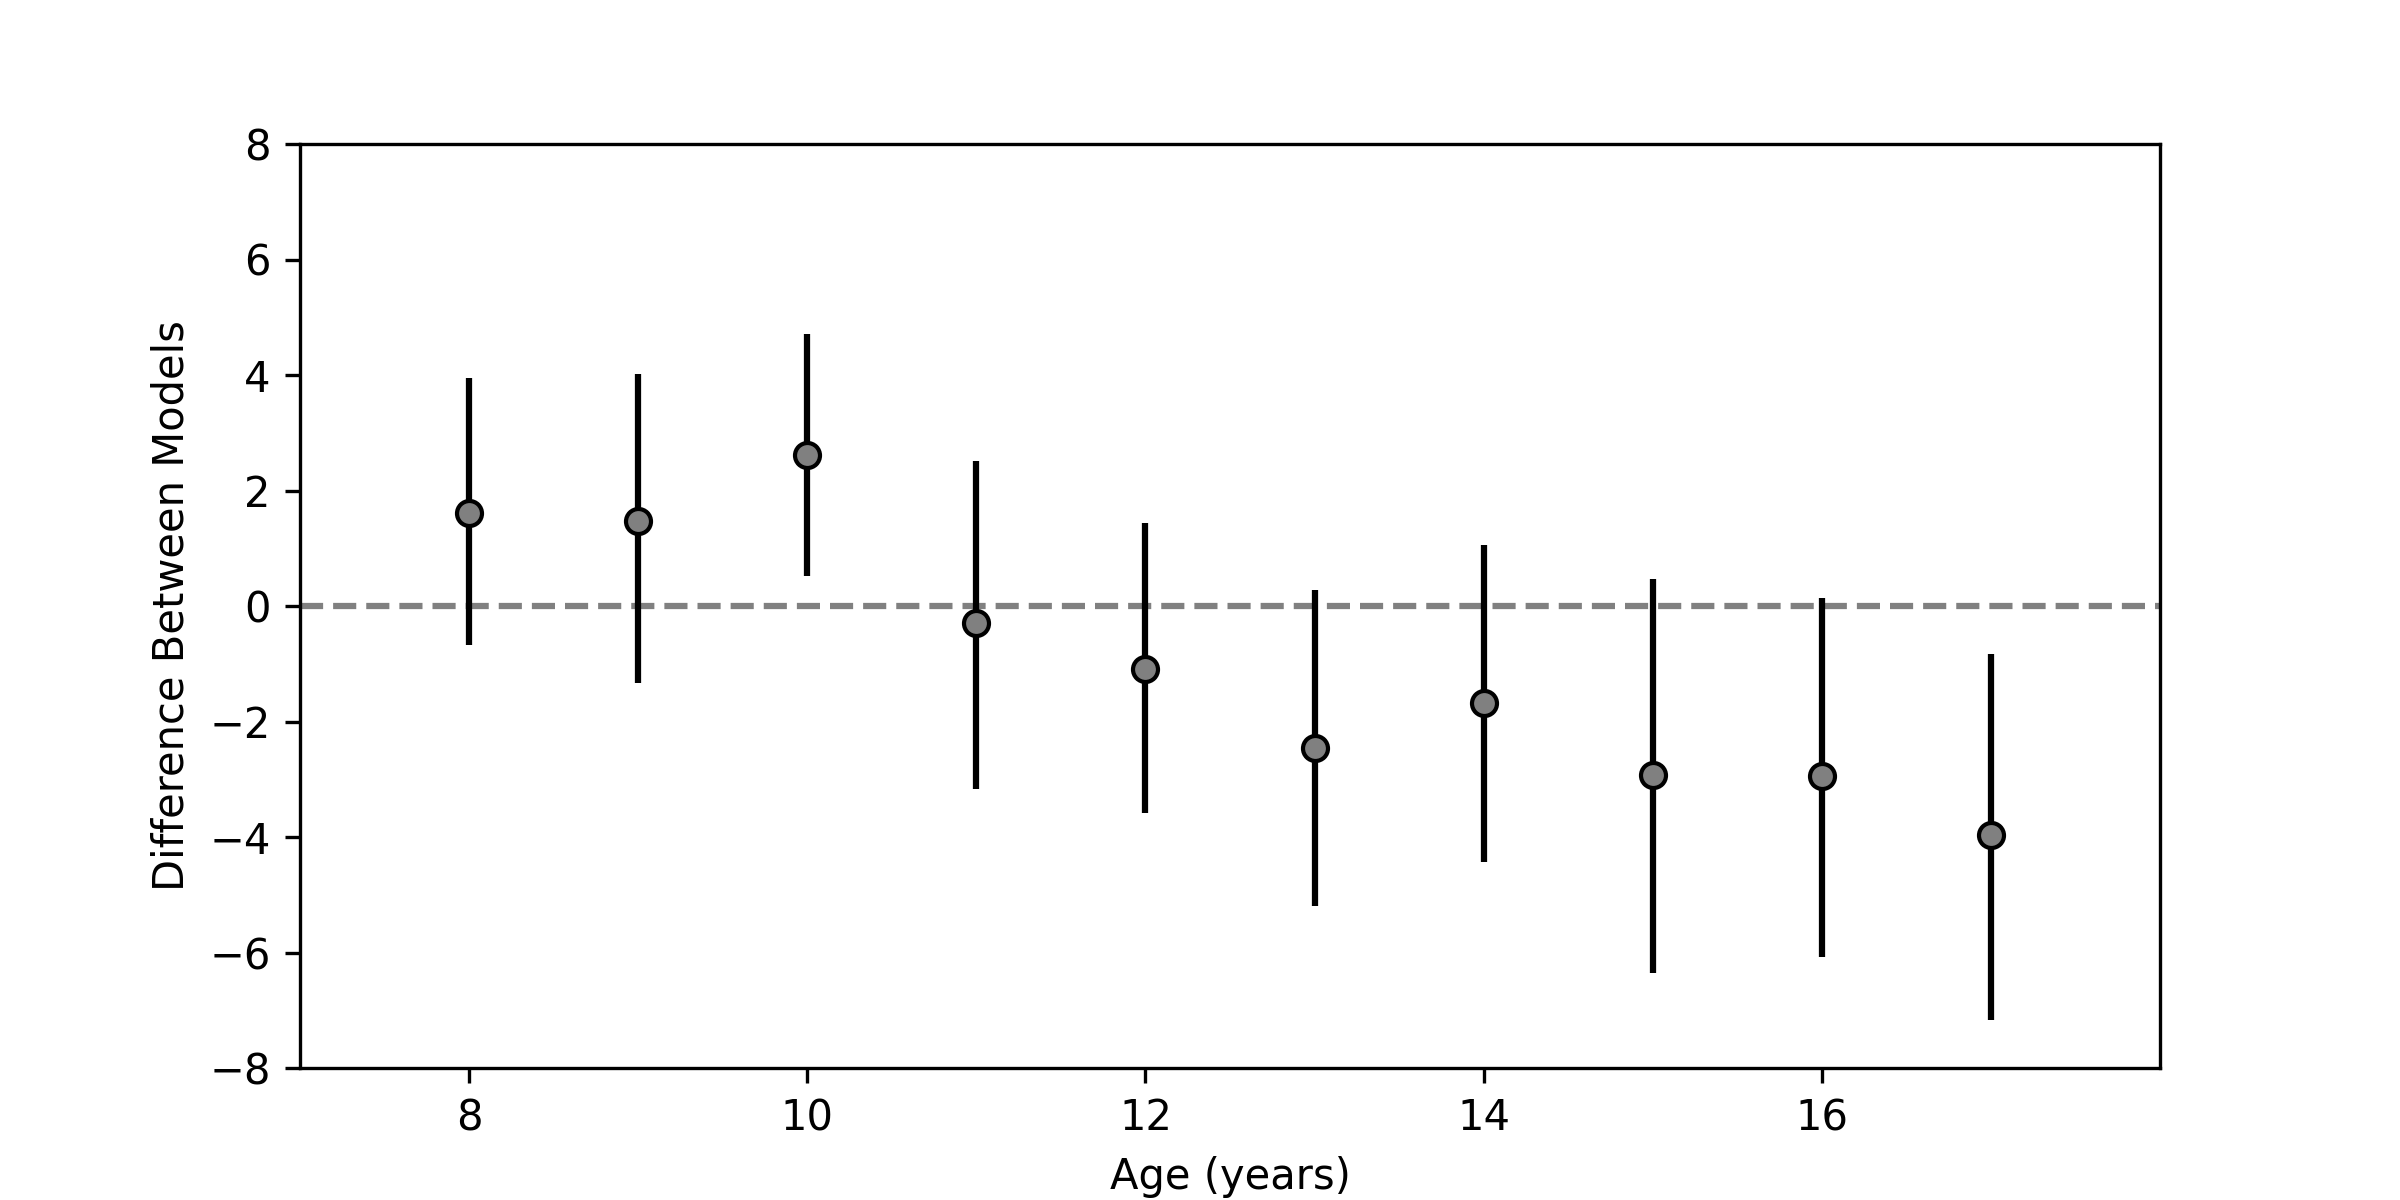
\includegraphics[width=0.9\linewidth]{images/diagnostic_plot2.png}
	\end{center}
\end{frame}

\end{document}